\section[Introduction]{Introduction}
\subsection[Production Lines and Handling Types]{Production Lines and Handling Types}
\begin{frame}
	%\frametitle{Production Lines}   
	\begin{columns}[c]
		\column{.7\textwidth}  % slides are 3in high by 5in wide
		\hspace{-1.2cm}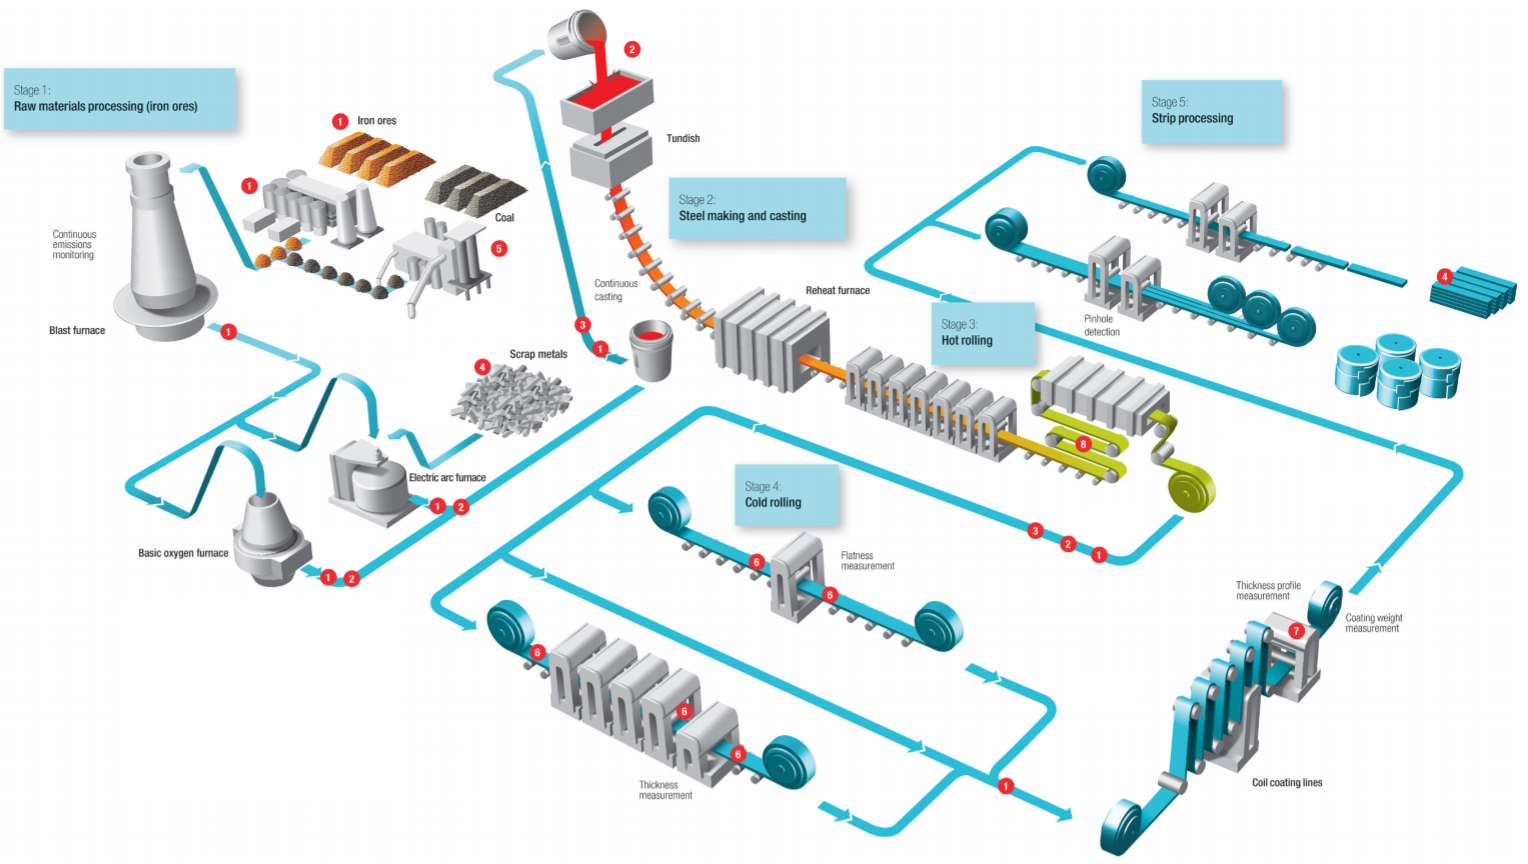
\includegraphics[width=11cm]{../images/steel-production-steps.png}
		\column{.3\textwidth}
		%\hspace{6cm}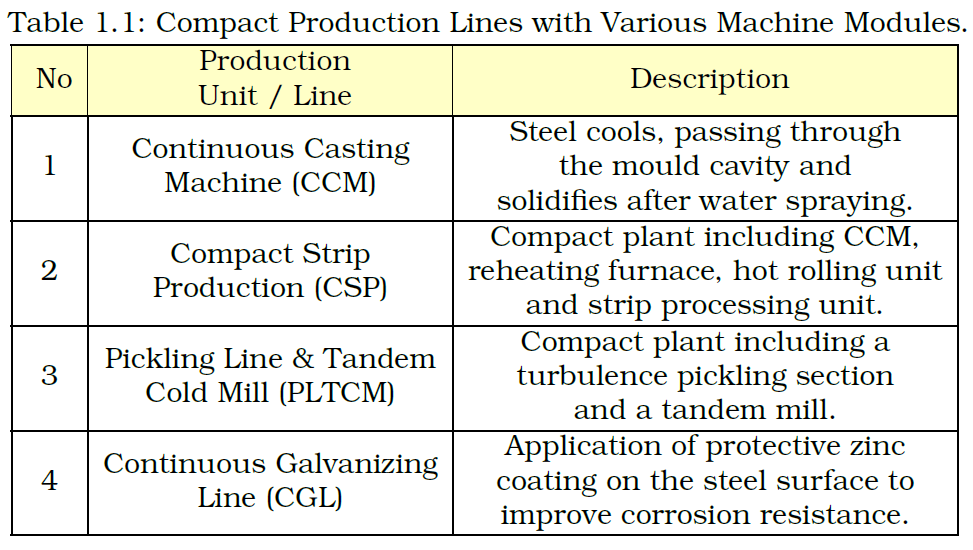
\includegraphics[height=3.7cm]{../tables/production_lines.png}
	\end{columns}
\end{frame}
\begin{frame}
	\begin{columns}[c]
		\column{.7\textwidth}  % slides are 3in high by 5in wide
		\hspace{-1.2cm}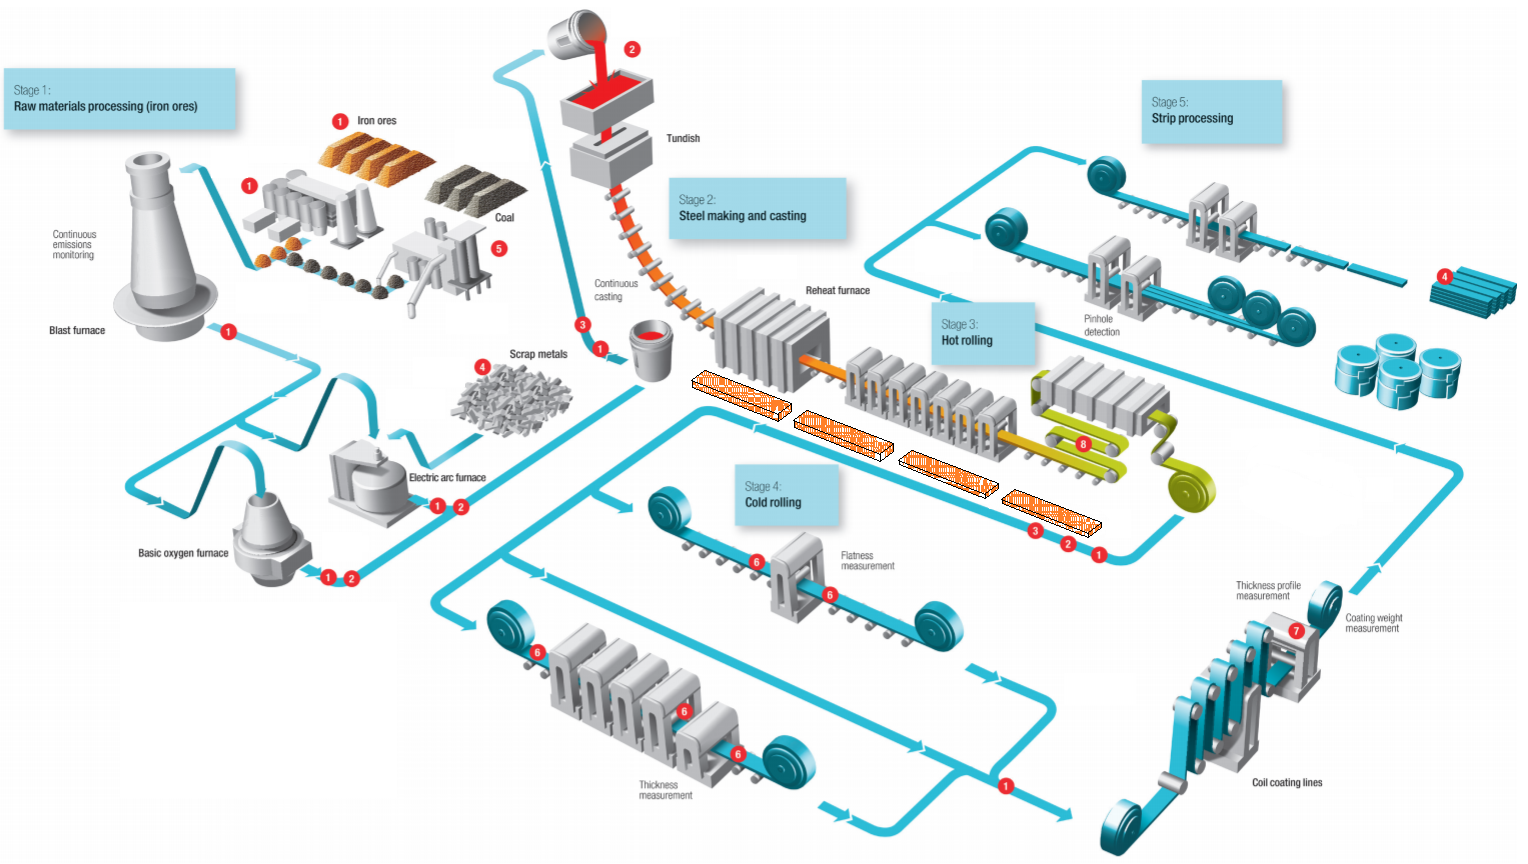
\includegraphics[width=11cm]{../tables/steel-production-steps_2.png}
		\column{.3\textwidth}
		%\hspace{6cm}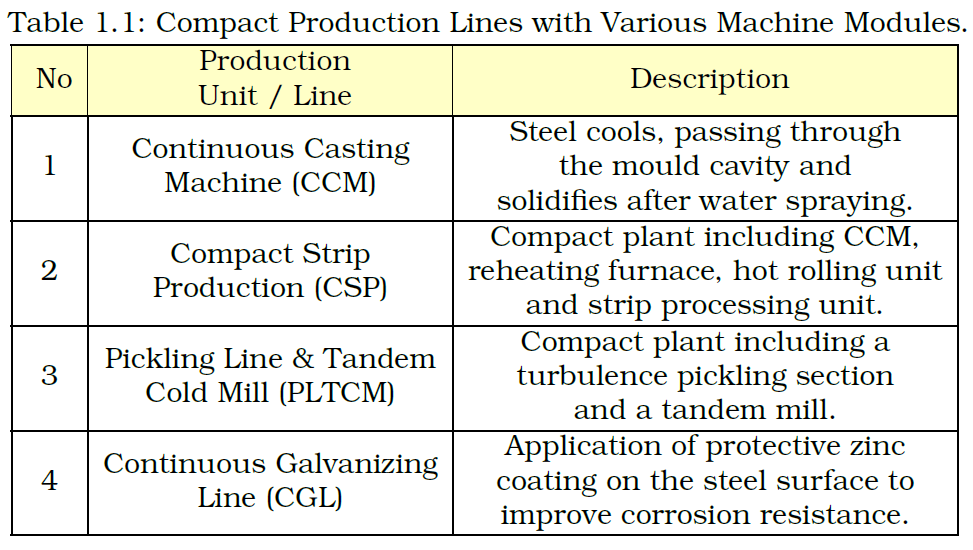
\includegraphics[height=3.7cm]{../tables/production_lines.png}
	\end{columns}
\end{frame}
\begin{frame}
	\begin{columns}[c]
		\column{.7\textwidth}  % slides are 3in high by 5in wide
		\hspace{-1.2cm}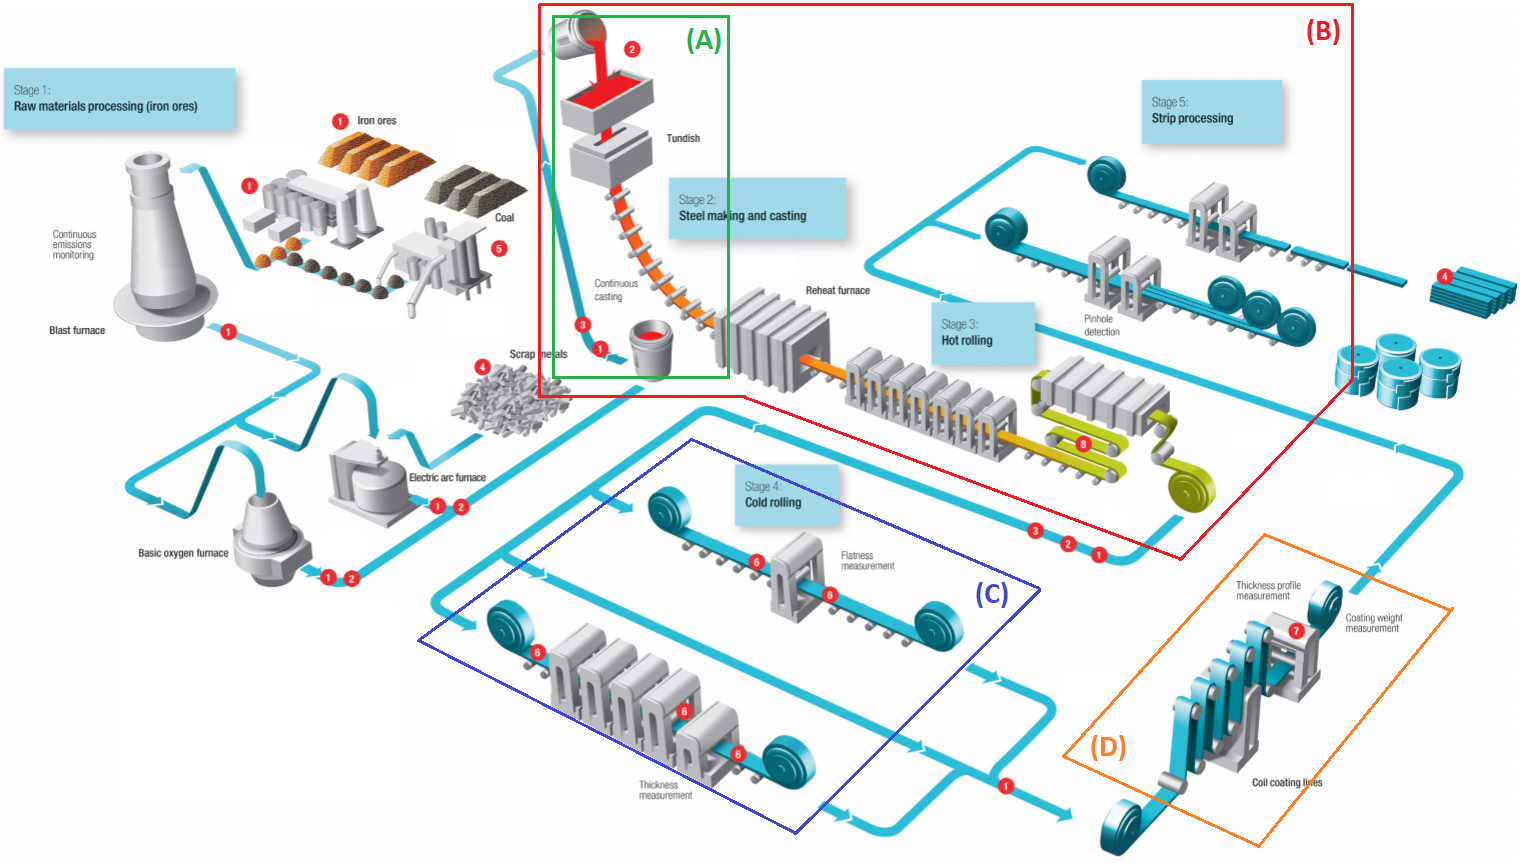
\includegraphics[width=11cm]{../images/steel-production-steps_old.png}
		\column{.3\textwidth}
		\hspace{6cm}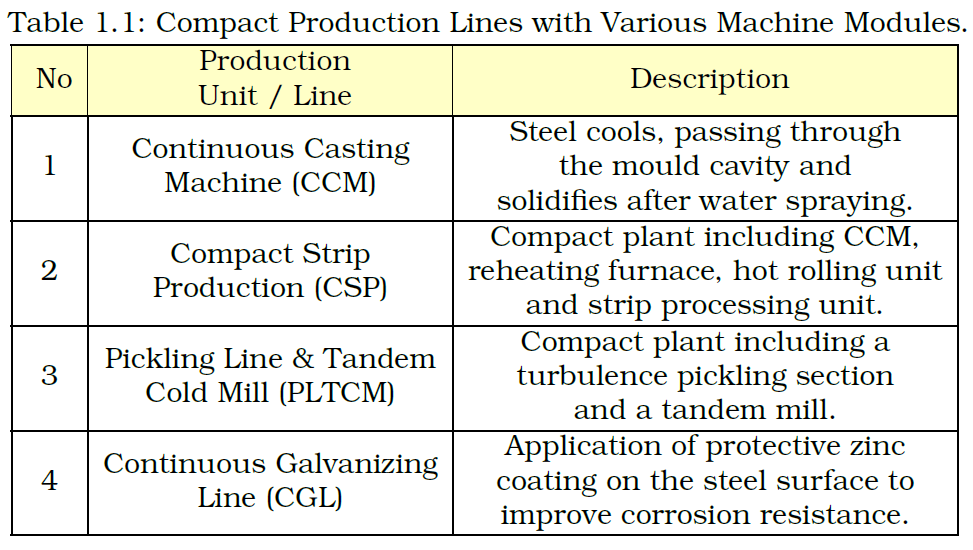
\includegraphics[height=3.7cm]{../tables/production_lines.png}
	\end{columns}
\end{frame}
\begin{frame}
	\begin{columns}[c]
		\column{.7\textwidth}  % slides are 3in high by 5in wide
		\hspace{-1.2cm}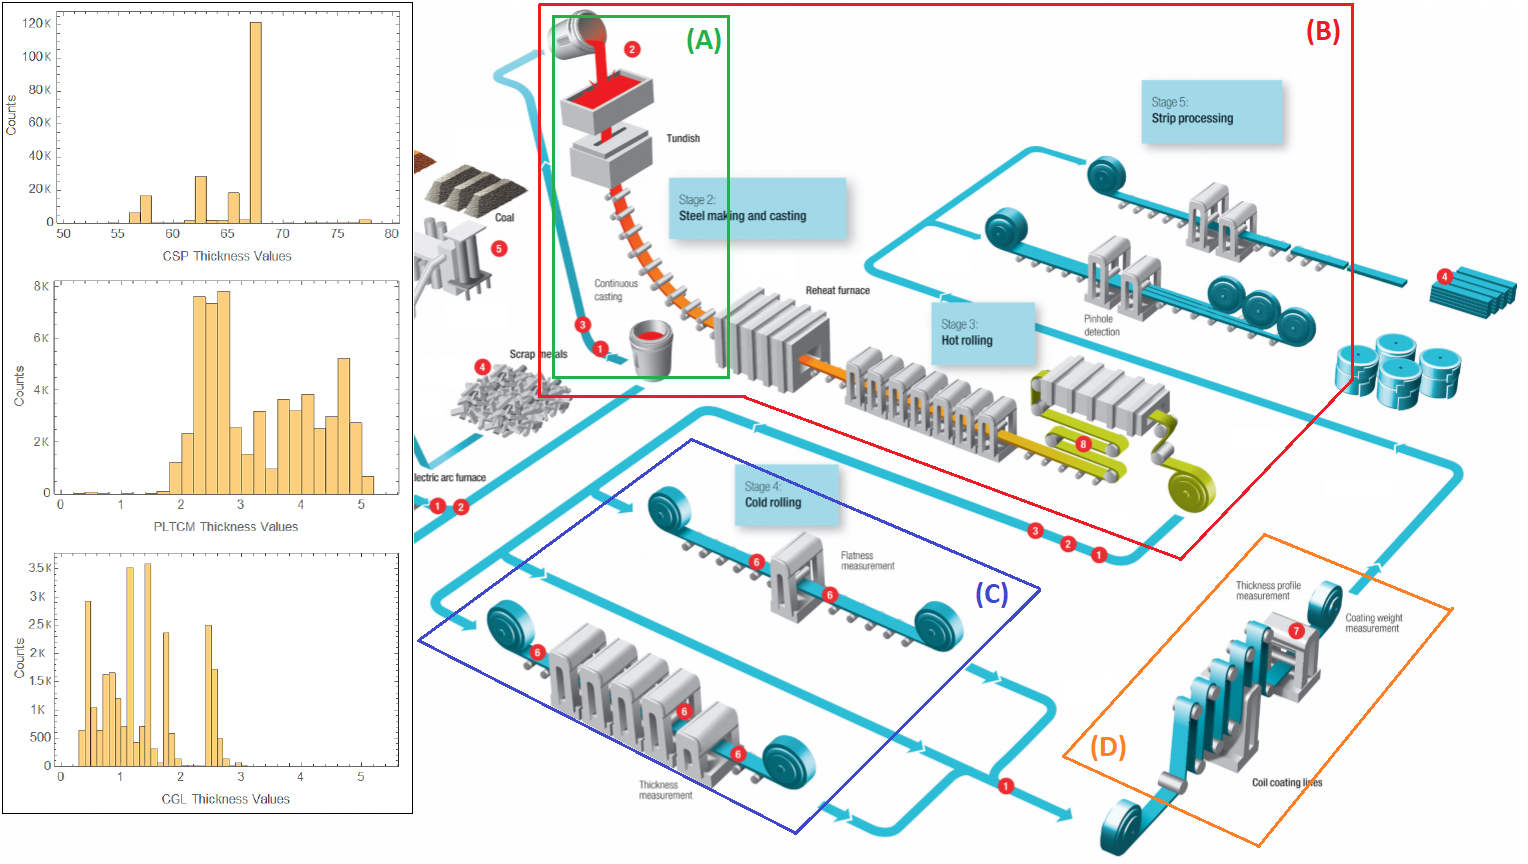
\includegraphics[width=11cm]{../tables/steel-production-steps_old_2.png}
		\column{.3\textwidth}
		\hspace{6cm}\centering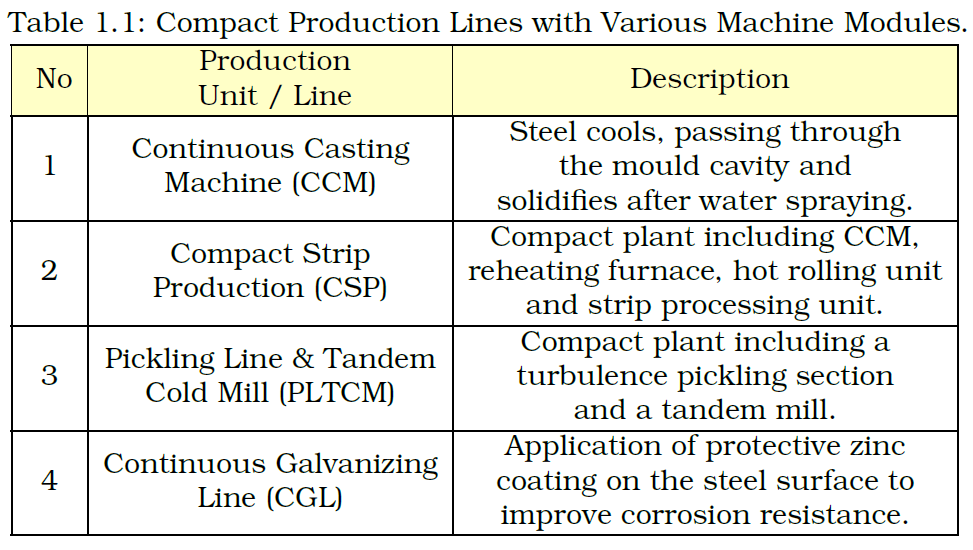
\includegraphics[height=3.7cm]{../tables/production_lines.png}
	\end{columns}
\end{frame}
\begin{frame}
	\begin{columns}[c]
		\column{.7\textwidth}  % slides are 3in high by 5in wide
		\hspace{-1.2cm}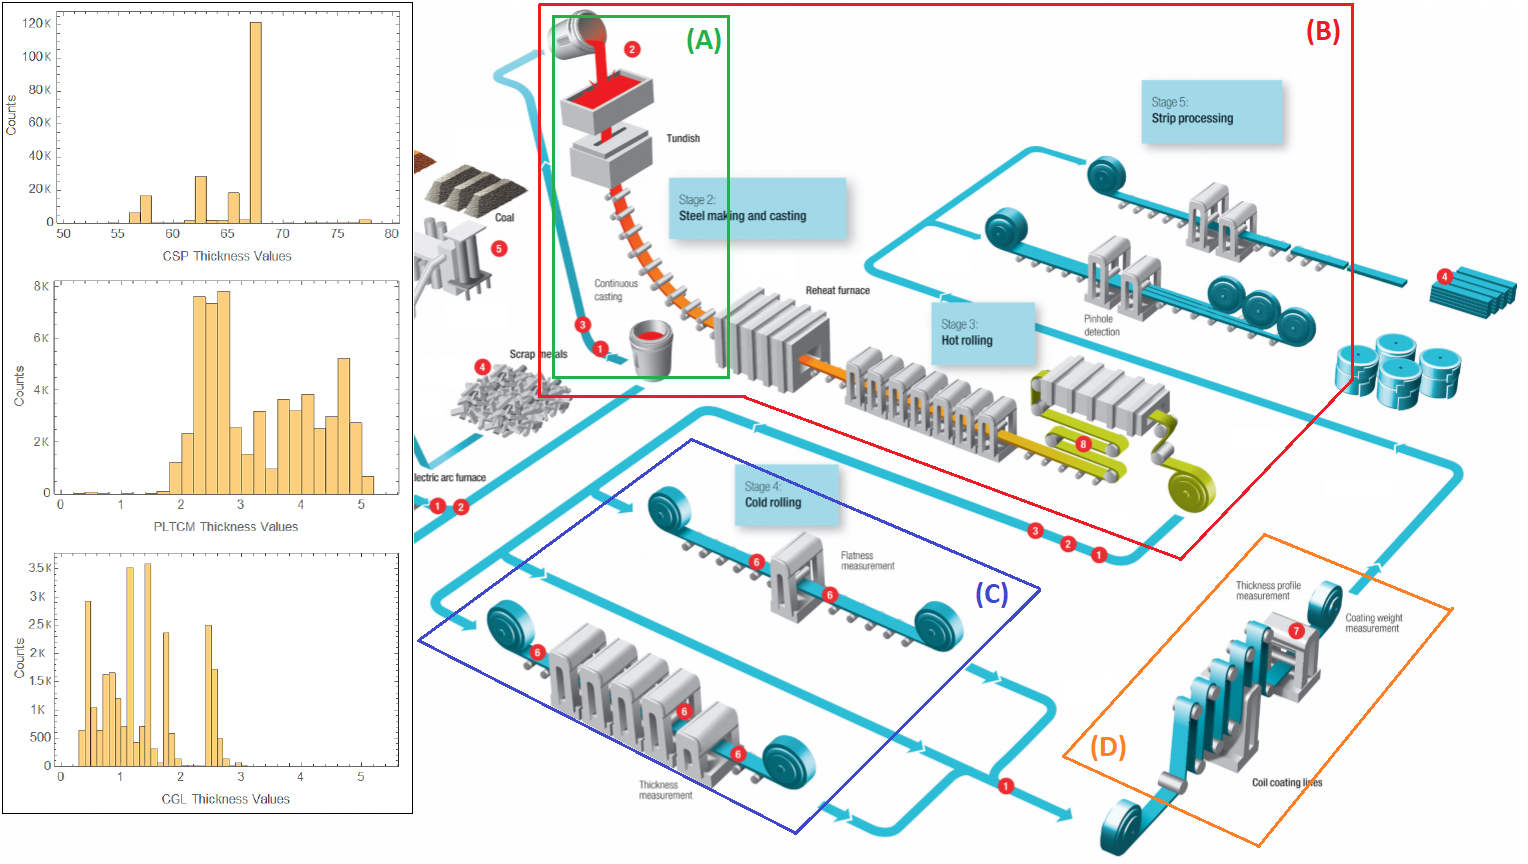
\includegraphics[width=11cm]{../tables/steel-production-steps_old_2.png}
		\column{.3\textwidth}
		\hspace{6cm}\centering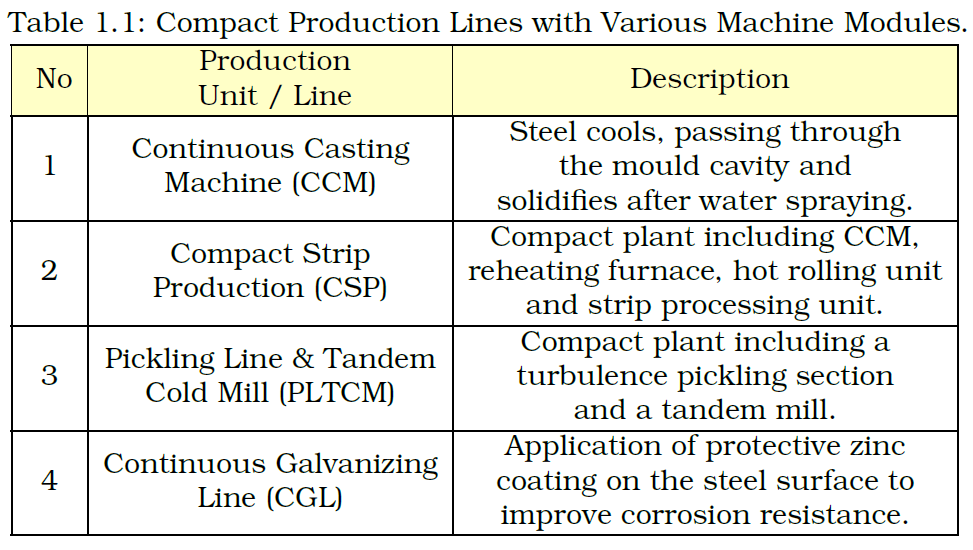
\includegraphics[height=3.7cm]{../tables/production_lines.png}
		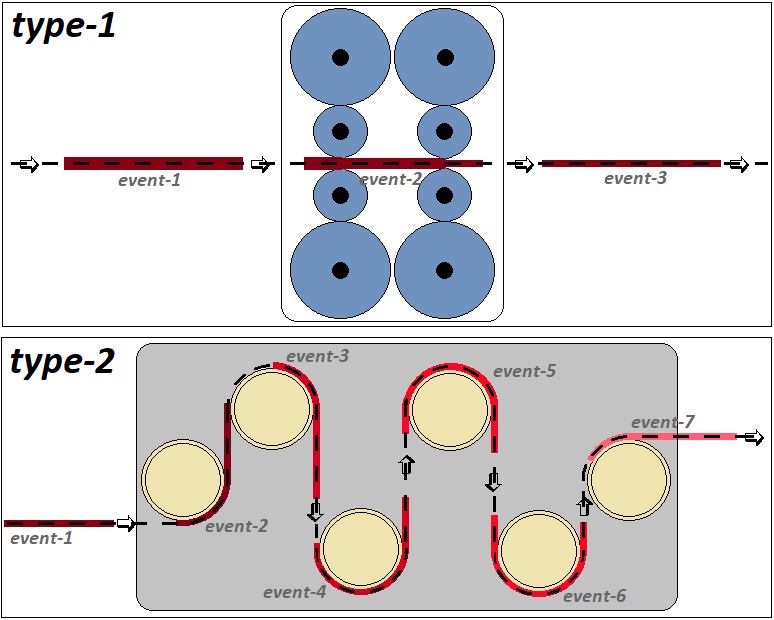
\includegraphics[width=\linewidth]{../tables/production_lines_handling_types_2.png}
	\end{columns}
\end{frame}
%\note[enumerate]       % Add notes to yourself that will be displayed when
%{                      % typeset with the notes or notesonly class options